\documentclass[../Master.tex]{subfiles}
\providecommand{\master}{..}
\begin{document}
For an action schema $A$, $\mathbb{P}_A$ is the set of all fluent predicates in the domain that can be applied with the arguments of $A$.
\[
    \mathbb{P}_A = \left\{
        p \left( x_1, \dots, x_{|p|} \right)
        \; | \; \left\{ x_1, \dots, x_{|p|} \right\} \subseteq params(A)
    \right\}
\]

\begin{figure}
    \centering
    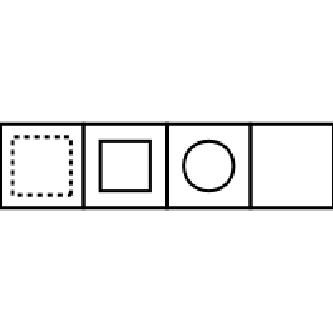
\includegraphics[scale=0.7]{../Graphics/sokoSmall}
    \caption{\label{fig:sokoSmall} Sokoban state with only one applicable \texttt{move-h} action. The tiles are named $t_1 \dots t_4$, from left to right. The crate object is named $c$.}
\end{figure}

We will now consider the problem of learning the preconditions of an action schema $A$.

In \cite{Walsh2008}, the authors suggest maintaining a set of all possible conjunctions of $k$ or less predicates (where $k$ is the maximal number of predicates allowed in action schema preconditions), and --- on action failure --- marking the conjunctions predicting that the action would have succeeded as disproven.

We propose a solution where individual predicates are proven and disproven to be preconditions based on the following observations:
\begin{itemize}
    \item When $a$ succeeds, there are predicates which, if they had been preconditions, would have caused failure. These can be immediately disproven to be preconditions.
    \item When $a$ fails, there are a number of predicates which could be responsible for the failure if they are preconditions. Although it is indeterminable which of them are preconditions and which are not, this information can be saved and analysed later, when more information is available.
\end{itemize}

In the following we will analyse how the aforementioned predicate sets can be deduced from a single state transition, and later discuss how knowledge obtained from earlier state transitions can be used to prove predicates to be preconditions.

\begin{example}[Sokoban example] \label{ex:ncp:sokobanSetup}
    As a running example, we will once again use the sokoban domain, where the environment starts in the following state (visualized in figure \ref{fig:sokoSmall}):
    \begin{equation*}
        s_0 =
        \left\{
            \begin{gathered}
                \texttt{sokobanAt}(t_3), \texttt{at}(b, t_2), \texttt{goal}(t_1), \\
                \texttt{clear}(t_1), \texttt{clear}(t_4), \\
                \texttt{hAdj}(t_1, t_2), \texttt{hAdj}(t_2, t_3),
                \texttt{hAdj}(t_3, t_4), \\
                \texttt{hAdj}(t_2, t_1), \texttt{hAdj}(t_3, t_2),
                \texttt{hAdj}(t_4, t_3)
            \end{gathered}
        \right\}
    \end{equation*}

    From this state, we will analyse the outcomes of different applications of the \texttt{move-h} action (presented in section \ref{sec:nc:sokobanExample}), whose preconditions are reprinted below:

    \begin{align*}
        P_{\texttt{move-h}}^+ &= \left\{
            \texttt{sokobanAt}(from), \texttt{clear}(to), \texttt{hAdj}(from, to)
            \right\} \\
        P_{\texttt{move-h}}^- &= \emptyset
    \end{align*}

    As can be seen, there is only one applicable \texttt{move-h} action in state $s_0$, namely $\texttt{move-h}(t_3,t_4)$. As the agent is unaware of this fact, it may apply other $\texttt{move-h}$ actions, which will all fail. The only information available to it is that both the positive and negative preconditions are subsets of $\mathbb{P}_{\texttt{move-h}}$, since no other predicate can be a precondition due to the scoping rule.

    \begin{equation*}
    \mathbb{P}_{\texttt{move-h}} =
    \left\{
        \begin{gathered}
            \texttt{sokobanAt}(to), \texttt{sokobanAt}(from), \\
            \texttt{clear}(to), \texttt{clear}(from), \\
            \texttt{goal}(to), \texttt{goal}(from), \\
            \texttt{vAdj}(from, to), \texttt{vAdj}(to, from), \\
            \texttt{vAdj}(from, from), \texttt{vAdj}(to, to), \\
            \texttt{hAdj}(from, to), \texttt{hAdj}(to, from), \\
            \texttt{hAdj}(from, from), \texttt{hAdj}(to, to), \\
            \texttt{at}(from, to), \texttt{at}(to, from)
        \end{gathered}
    \right\}
    \end{equation*}
\end{example}

\subsection{Learning from a transition}
\subfile{\master/NonConditional/Preconditions/Transition}

\subsection{Using prior knowledge}
\subfile{\master/NonConditional/Preconditions/PriorKnowledge}

\end{document}
